\section{Transformations}

Transformations map geometry. In the graphics pipeline this is mostly used for changing positions and orientations for objects, projecting them to the screen and animating objects.

\subsection{2D Transformations}
\begin{itemize}
	\item Translation - note that translation is not linear as it corresponds to vector addition
	$$\begin{pmatrix}
		x' \\ y'
	\end{pmatrix} = \begin{pmatrix}
		x \\ y
	\end{pmatrix} + \begin{pmatrix}
		t_x \\ t_y
	\end{pmatrix}$$
	
	\item Scaling
	$$\begin{pmatrix}
		x' \\ y'
	\end{pmatrix} = \begin{bmatrix}
		s_x & 0 \\ 0 & s_y
	\end{bmatrix} \cdot \begin{pmatrix}
		x \\ y
	\end{pmatrix}$$
	
	\item Rotation
	$$\begin{pmatrix}
		x' \\ y'
	\end{pmatrix} = \begin{bmatrix}
		\cos \theta & - \sin \theta \\ \sin \theta & \cos \theta
	\end{bmatrix} \cdot \begin{pmatrix}
		x \\ y
	\end{pmatrix}$$
\end{itemize}

Affine maps are linear in homogeneous coordinates (adding one dimension). This allows us to perform translations as a linear operation ($p' = \textbf T p$).

\begin{itemize}
	\item Translation	
	$$\textbf T = \begin{bmatrix}
		1 & 0 & t_x \\ 0 & 1 & t_y \\ 0 & 0 & 1
	\end{bmatrix}$$
	
	\item Scaling
	$$\textbf S = \begin{bmatrix}
		s_x & 0  & 0\\ 0 & s_y & 0 \\ 0 & 0 & 1
	\end{bmatrix}$$
	
	\item Rotation
	$$\textbf R = \begin{bmatrix}
		\cos \theta & - \sin \theta & 0 \\ \sin \theta & \cos \theta & 0 \\ 0 & 0 & 1
	\end{bmatrix}$$
	
	\item Shear along $x$-axis ($a$) and along the $y$-axis ($b$)
	$$\textbf{SH} = \begin{bmatrix}
		1 & a  & 0\\ 0 & 1 & 0 \\ 0 & 0 & 1
	\end{bmatrix} \qquad \textbf{SH} = \begin{bmatrix}
		1 & 0  & 0\\ b & 1 & 0 \\ 0 & 0 & 1
	\end{bmatrix}$$
\end{itemize}

When transforming back from the homogeneous coordinates it is important to divide by the last value. We can easily combine multiple transformation by taking the matrix product.


\subsection{3D Transformations}

We also want to use homogeneous coordinates in the 3D space. 
\begin{itemize}
	\item Translation	
	$$\textbf T = \begin{bmatrix}
		1 & 0 & 0 & t_x \\ 0 & 1 & 0 & t_y \\ 0 & 0 & 1 & t_z \\ 0 & 0 & 0 & 1
	\end{bmatrix}$$
	
	\item Scaling
	$$\textbf S = \begin{bmatrix}
		s_x & 0 & 0 & 0 \\ 0 & s_y & 0 & 0 \\ 0 & 0 & s_z & 0 \\ 0 & 0 & 0 & 1
	\end{bmatrix}$$
	
	\item Rotation - this is \textbf{not commutative} anymore!
	$$\textbf R_x = \begin{bmatrix}
		1 & 0 & 0 & 0 \\ 0 & \cos \theta & - \sin \theta & 0 \\ 0 & \sin \theta & \cos \theta & 0 \\ 0 & 0 & 0 & 1
	\end{bmatrix}$$
	$$\textbf R_y = \begin{bmatrix}
		\cos \theta & 0 & \sin \theta & 0 \\ 0 & 1 & 0 & 0 \\ -\sin \theta & 0 & \cos \theta & 0 \\ 0 & 0 & 0 & 1
	\end{bmatrix}$$
	
	$$\textbf R_z = \begin{bmatrix}
		\cos \theta & - \sin \theta & 0 & 0 \\ \sin \theta & \cos \theta & 0 & 0 \\ 0 & 0 & 1 & 0 \\ 0 & 0 & 0 & 1
	\end{bmatrix}$$
	
	\item Shear parallel to the principal planes
	$$\textbf{SH}_{xy} = \begin{bmatrix}
		1 & 0 & sh_x & 0\\ 0 & 1 & sh_y & 0 \\ 0 & 0 & 1 & 0 \\ 0 & 0 & 0 & 1
	\end{bmatrix}$$
	$$\textbf{SH}_{xz} = \begin{bmatrix}
		1 & sh_x & 0 & 0\\ 0 & 1 & 0 & 0 \\ 0 & sh_z & 1 & 0 \\ 0 & 0 & 0 & 1
	\end{bmatrix}$$
	
	$$\textbf{SH}_{yz} = \begin{bmatrix}
		1 & 0 & 0 & 0\\ sh_y & 1 & 0 & 0 \\ sh_z & 0 & 1 & 0 \\ 0 & 0 & 0 & 1
	\end{bmatrix}$$
\end{itemize}


\subsection{Coordinate Systems}

A coordinate system represents a point / vector as a linear combination of orthonormal basis vectors.
$$p = p_x x + p_y y + p_z z$$

A change of coordinate systems consists of a combination of translation and rotation:
$$p' = \textbf T \textbf R p = \begin{bmatrix}
	r_1 & r_2 & r_3 & t \\
	0 & 0 & 0 & 1
\end{bmatrix} \begin{pmatrix}
	p_x \\ p_y \\ p_z \\ 1
\end{pmatrix}$$

We are also interested in how the surface normal $n$ is transformed. Given a transformation $p' = \textbf M p$ the surface normal is transformed by $n' = (\textbf M'{-1})^\top n$.


\subsection{Projection}

When we want to go from 3D space to 2D space, e.g. when projecting to screen space, we have to think about perspective. We differentiate two types of projection.
\begin{center}
	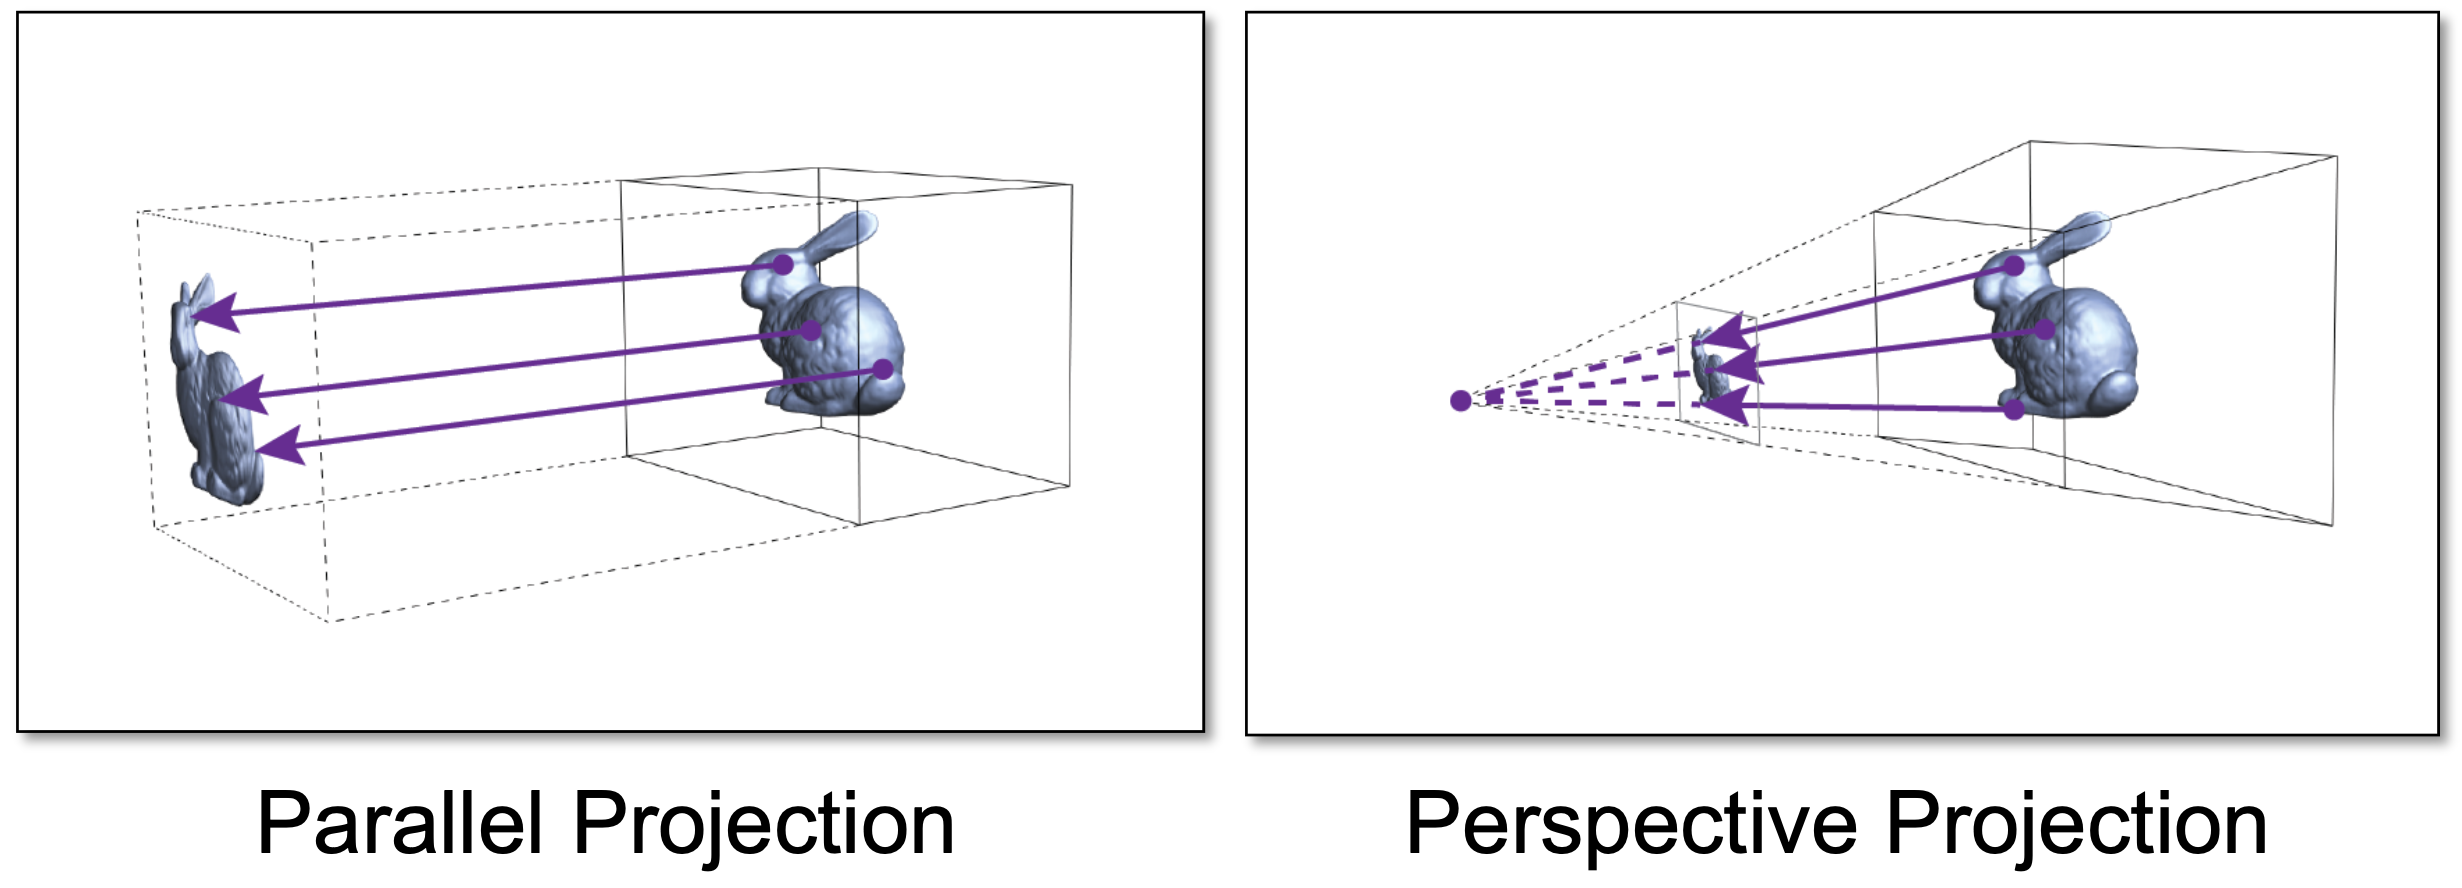
\includegraphics[width=\linewidth]{projection.png}
\end{center}

Perspective projection corresponds to how a camera would see an object. In perspective projection the lines seem to converge in some point, these points are called vanishing points. If we have more than three vanishing points we have multiple center of projection.

\subsubsection{Mathematics of Perspective Projection}

If the camera plane is defined by the $x$ and $y$ axis, i.e. the coordinate system is aligned with the $z$ axis, the math behind the projection is easy. This is the reason we first transform from world coordinates to camera coordinates. For a given focal distance $d$, the projection is then given by:
$$\textbf M p = \begin{bmatrix}
	1 & 0 & 0 & 0 \\
	0 & 1 & 0 & 0 \\
	0 & 0 & 1 & 0 \\
	0 & 0 & 1/d & 0
\end{bmatrix} \begin{pmatrix}
	x \\ y \\ z \\ 1
\end{pmatrix} = \begin{pmatrix}
	x \\ y \\ z \\ z / d
\end{pmatrix}$$

If we transform this back to non homogeneous space, we end up with:
$$\begin{pmatrix}
	dx / z \\ dy / z \\ d
\end{pmatrix}$$

\subsubsection{Mathematics of Parallel Projection}

This is a lot simpler and corresponds to:
$$\textbf M = \begin{bmatrix}
	1 & 0 & 0 & 0 \\
	0 & 1 & 0 & 0 \\
	0 & 0 & 0 & 0 \\
	0 & 0 & 0 & 1
\end{bmatrix}$$



